%%%%%%%%%%%%%%%%%%%%%%%%%%%%%%%%%%%%%%%%%%%%%%%%%%%%%%%%%%%%%%%%%%%%%%%%%%%%%%%%%%%%%%%%%%%
\subsubsection*{Delineamento Procedimental da Revisão Sistemática}

\subsubsection*{Estratégia de busca e extração dos estudos}

A revisão sistemática foi conduzida seguindo as diretrizes do PRISMA (\textit{Preferred Reporting Items for Systematic Reviews and Meta-Analyses}) para garantir transparência e reprodutibilidade metodológica. A busca foi realizada nas principais bases de dados científicas com acesso periódico CAPES: Scopus (Elsevier), \textit{Web of Science} (Clarivate Analytics), IEEE Xplore Digital Library, ACM Digital Library e PubMed. A estratégia de busca foi fundamentada na intersecção de três domínios temáticos principais: (i) técnicas de machine learning e inteligência artificial; (ii) estudos etnográficos e conhecimentos tradicionais; e (iii) agroecologia e sistemas tradicionais de manejo.

Os descritores foram estruturados utilizando terminologia controlada em língua inglesa, articulados por operadores booleanos (AND, OR, NOT) conforme protocolo estabelecido por \citeonline{Moher2009}, abrangendo publicações dos últimos 10 anos (2014-2024) para capturar o estado da arte em machine learning aplicado a estudos etnográficos. A estratégia de busca foi construída seguindo a lógica: 

\textbf{("machine learning" OR "artificial intelligence" OR "deep learning" OR "natural language processing" OR "ensemble methods" OR "convolutional neural networks") AND ("traditional knowledge" OR "indigenous knowledge" OR "ethnography" OR "participatory research" OR "community-based research") AND ("agroecology" OR "sustainable agriculture" OR "traditional farming" OR "ecological knowledge" OR "biodiversity conservation")}.

Os critérios de inclusão contemplaram: artigos completos publicados em periódicos revisados por pares, escritos em inglês, português ou espanhol, que apresentem aplicações de técnicas computacionais em estudos etnográficos ou mapeamento de conhecimentos tradicionais relacionados à agricultura e conservação ambiental. Os descritores primários deveriam estar presentes nos campos: título, resumo ou palavras-chave dos manuscritos.

\subsubsection*{Rodada 1: Triagem e seleção automática}

\subsubsection*{\textit{Classificação automática por relevância temática}}

A triagem inicial dos estudos foi realizada utilizando uma abordagem híbrida que combina classificação automática e revisão manual. Para a fase de seleção automática, foi empregado o software StArt (\textit{State of the Art through Systematic Review}) \cite{Hernandes2012}, implementando o Sistema de Classificação Automática de Citações por Pontuação (SCAS). O SCAS opera em duas fases distintas: classificação por pontuação baseada na frequência de descritores-chave e posicionamento hierárquico dos artigos em quadrantes de relevância.

Na primeira fase, o algoritmo atribui pontuações diferenciadas baseadas na localização dos descritores temáticos: 5 pontos para ocorrências no título, 3 pontos no resumo e 2 pontos nas palavras-chave. Os descritores específicos utilizados incluíram: \textit{Machine Learning, Deep Learning, Natural Language Processing, Traditional Knowledge, Indigenous Knowledge, Ethnography, Agroecology, Participatory Research, Conservation, Biodiversity} e \textit{Sustainable Agriculture}.

A segunda fase emprega o método de Posicionamento Hierárquico de Pontos (HiPP), desenvolvido por \citeonline{Paulovich2008}, que categoriza os artigos em quatro quadrantes baseados em dois eixos: relevância temática e qualidade metodológica. A classificação segue as seguintes categorias:

\begin{enumerate}
  \item \textbf{Categoria 1 (Automática):} Artigos posicionados nos quadrantes Q1 (alta relevância, alta qualidade) são automaticamente incluídos, enquanto artigos em Q4 (baixa relevância, baixa qualidade) são automaticamente excluídos da análise;

  \item \textbf{Categoria 2 (Revisão Manual):} Artigos nos quadrantes Q2 (alta relevância, qualidade moderada) e Q3 (relevância moderada, alta qualidade) são submetidos à avaliação manual por dois revisores independentes para decisão final de inclusão ou exclusão.
\end{enumerate}

A Figura \ref{fig:1} ilustra a distribuição dos quadrantes e categorias utilizadas no processo de classificação hierárquica.

\begin{figure}[H]
  \centering
  \caption{Quadrantes e categorias adotadas no posicionamento hierárquico de pontos para estudos de machine learning em etnografia}
  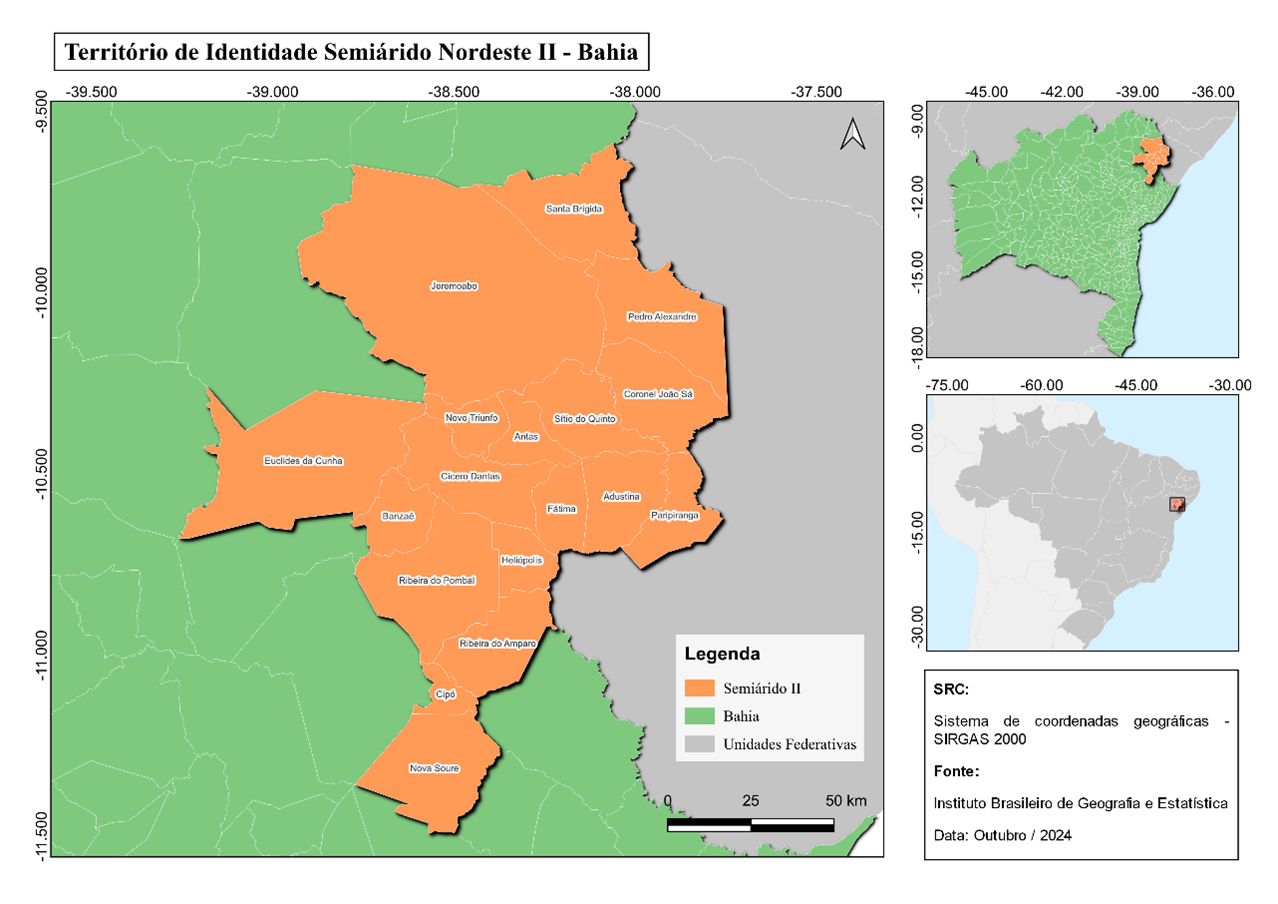
\includegraphics[scale=0.5]{Imagens/fig_1.png}
  \fonte{\textbf{Elaborado pelos autores} (2024)}
  \label{fig:1}
\end{figure}

Para completar a extração dos artigos classificados nos quadrantes Q2 e Q3, foi realizada leitura completa de títulos, resumos e palavras-chave, com foco na identificação de aplicações efetivas de técnicas computacionais em contextos etnográficos ou de mapeamento participativo de conhecimentos tradicionais.

\subsubsection*{\textit{Seleção manual especializada}}

A seleção manual foi conduzida por dois revisores independentes, ambos com experiência em machine learning e estudos etnográficos. Os critérios de inclusão/exclusão foram estruturados considerando a especificidade temática da intersecção entre inteligência artificial e conhecimentos tradicionais, conforme apresentado na Tabela \ref{tab:1}.

\begin{table}[H]
  \centering
  \caption{Critérios de Inclusão/Exclusão para estudos de machine learning em etnografia}
  \label{tab:1}
  \resizebox{\columnwidth}{!}{%
    \begin{tabular}{lc}
      \hline
      \multicolumn{1}{c}{\textbf{Critérios}}                     & \textbf{Classificação}  \\ \hline
      Apresenta aplicação direta de ML/IA em estudos etnográficos                  & Inclusão (I)               \\
      Aborda mapeamento computacional de conhecimentos tradicionais             & Inclusão (I)               \\
      Integra metodologias participativas com técnicas computacionais                 & Inclusão (I)               \\
      Foca exclusivamente em aspectos técnicos sem contexto etnográfico                  & Exclusão (E)               \\
      Não apresenta inovação metodológica na intersecção ML-etnografia                  & Exclusão (E)               \\
      Carece de validação em comunidades tradicionais ou indígenas                          & Exclusão (E)               \\
      Não demonstra reprodutibilidade dos algoritmos propostos & Exclusão (E)               \\
      Constitui revisão bibliográfica sem contribuição metodológica original                              & Exclusão (E)               \\
      Baixa aderência aos três domínios temáticos fundamentais                & Exclusão (E)               \\ \hline
    \end{tabular}%
  }
\end{table}

Artigos que não atenderam pelo menos dois critérios de inclusão foram automaticamente excluídos. As discrepâncias entre avaliadores foram resolvidas através de consenso em reuniões estruturadas, com consulta a um terceiro revisor especialista quando necessário.

\subsubsection*{Rodada 2: Extração de dados temáticos}

\subsubsection*{\textit{Categorização por domínios tecnológicos}}

Para a classificação qualitativa dos artigos selecionados, foi desenvolvido um sistema de categorização baseado em três dimensões principais: (i) técnicas de machine learning empregadas; (ii) contexto etnográfico de aplicação; e (iii) nível de participação comunitária. Cada dimensão recebeu pontuação de 0 a 2 pontos, totalizando uma escala de 0 a 6 pontos por artigo.

\begin{enumerate}[label=(\alph*)]
\item \textbf{Técnicas de Machine Learning:} Classificação baseada na sofisticação algorítmica empregada: 2 pontos para técnicas avançadas (deep learning, ensemble methods, NLP transformers), 1 ponto para métodos intermediários (SVM, random forest, redes neurais simples), 0 pontos para técnicas básicas (regressão linear, clustering simples);

\item \textbf{Contexto Etnográfico:} Avaliação da profundidade da integração com estudos etnográficos: 2 pontos para estudos com trabalho de campo extensivo e validação comunitária, 1 ponto para aplicações com dados etnográficos secundários, 0 pontos para simulações ou dados sintéticos;

\item \textbf{Participação Comunitária:} Mensuração do nível de envolvimento das comunidades tradicionais: 2 pontos para metodologias genuinamente participativas com co-criação, 1 ponto para consulta comunitária estruturada, 0 pontos para abordagens unilaterais de pesquisa.
\end{enumerate}

A seleção desta rodada priorizou manuscritos que demonstrassem inovação metodológica na integração entre técnicas computacionais e abordagens etnográficas, com atenção especial para estudos que respeitassem princípios éticos de pesquisa com povos tradicionais.

\subsubsection*{\textit{Análise de qualidade metodológica}}

Para avaliação da qualidade metodológica dos estudos, foi adaptada a escala MMAT (\textit{Mixed Methods Appraisal Tool}) \cite{Hong2018} específicamente para estudos interdisciplinares envolvendo machine learning e etnografia. Os indicadores de qualidade (Tabela \ref{tab:2}) foram estruturados em uma escala Likert de 0 a 3 pontos: 0 (não atende), 1 (atende parcialmente), 2 (atende adequadamente), 3 (atende completamente).

\begin{table}[H]
  \centering
  \caption{Indicadores de qualidade metodológica para estudos ML-etnografia}
  \label{tab:2}
  \resizebox{\textwidth}{!}{%
    \begin{tabular}{lll}
      \hline
      \multicolumn{1}{c}{\textbf{Código}} & \multicolumn{1}{c}{\textbf{Indicador}}                             & \multicolumn{1}{c}{\textbf{Domínio}} \\ \hline
      RIG                                 & Rigor metodológico na coleta e processamento de dados etnográficos                      & Qualidade Etnográfica                         \\
      VAL                                 & Validação técnica dos algoritmos com métricas apropriadas                     & Qualidade Computacional                         \\
      ETI                                 & Aderência a protocolos éticos para pesquisa com comunidades tradicionais                               & Qualidade Ética                         \\
      REP                                 & Reprodutibilidade dos experimentos computacionais                                        & Qualidade Técnica                         \\
      INT                                 & Integração efetiva entre métodos quantitativos e qualitativos      & Qualidade Metodológica                         \\
      IMP                                 & Impacto e aplicabilidade dos resultados para as comunidades estudadas       & Qualidade Social                         \\
      DOC                                 & Documentação completa dos algoritmos e procedimentos etnográficos & Qualidade Documental                         \\
      GEN                                 & Generalizabilidade e transferibilidade dos métodos propostos                   & Qualidade Científica                         \\ \hline
    \end{tabular}%
  }
\end{table}

Artigos com pontuação total superior a 18 pontos (75\% da pontuação máxima) foram classificados como alta qualidade, entre 12-18 pontos como qualidade moderada, e abaixo de 12 pontos como baixa qualidade. Estudos de baixa qualidade foram excluídos das análises subsequentes.

\subsubsection*{Rodada 3: Análise bibliométrica e redes de colaboração}

Para análise da produtividade científica e identificação de redes de colaboração na intersecção entre machine learning e estudos etnográficos, foi aplicada a Lei de Lotka \cite{Lotka1926} para distribuição de autores, complementada por análise de cocitação e acoplamento bibliográfico. A análise de redes foi realizada utilizando o software VOSviewer \cite{VanEck2010}, considerando:

\begin{itemize}
\item Redes de coautoria entre pesquisadores;
\item Clusters temáticos baseados em palavras-chave;
\item Evolução temporal das publicações (2014-2024);
\item Distribuição geográfica e institucional dos estudos;
\item Identificação de periódicos centrais na área.
\end{itemize}

Esta análise permitiu mapear a estrutura da produção científica na área, identificando lacunas temáticas e oportunidades de pesquisa futura.

\subsubsection*{Rodada 4: Síntese qualitativa e quantitativa}

A síntese final integrou análise qualitativa temática com meta-análise quantitativa quando aplicável. Para identificação dos estudos mais relevantes, foi aplicado o princípio de Pareto (80/20) \cite{Pareto1964}, selecionando os 20\% dos artigos com maior pontuação combinada das rodadas anteriores, que representaram aproximadamente 80\% do impacto científico total do corpus analisado.

O somatório final considerou: (i) pontuação de relevância temática (Rodada 1); (ii) qualidade metodológica (Rodada 2); e (iii) impacto bibliométrico (Rodada 3). A distribuição dos pesos foi: 40\% para qualidade metodológica, 35\% para relevância temática e 25\% para impacto bibliométrico.

A Figura \ref{fig:2} apresenta o fluxograma completo do processo de revisão sistemática adaptado para estudos interdisciplinares de machine learning e etnografia.

\begin{landscape}
\begin{figure}[H]
  \centering
  \caption{Fluxograma da revisão sistemática para machine learning em estudos etnográficos}
  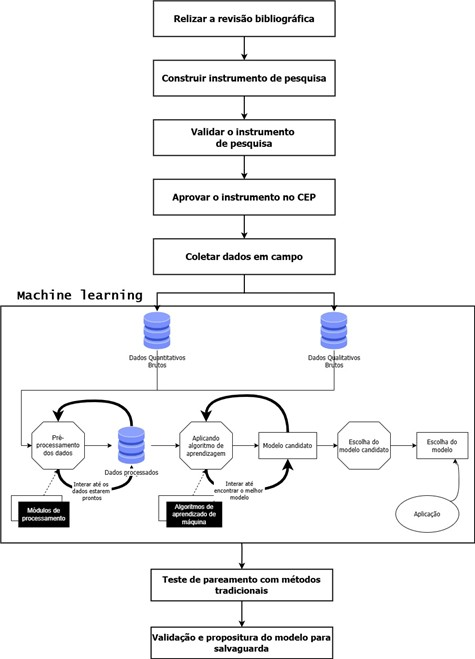
\includegraphics[scale=1.5]{Imagens/fig_2.jpg}
  \fonte{\textbf{Elaborado pelos autores} (2024)}
  \label{fig:2}
\end{figure}
\end{landscape}

A metodologia foi validada segundo os critérios AMSTAR-2 (\textit{Assessment of Multiple Systematic Reviews}) \cite{Shea2017}, garantindo conformidade com padrões de qualidade para revisões sistemáticas em áreas interdisciplinares emergentes.